\documentclass[a4paper, 11pt]{article}
\usepackage{comment} 
\usepackage{fullpage} 
\usepackage[spanish]{babel} 
\selectlanguage{spanish}
\usepackage[utf8]{inputenc}
\usepackage{float} 
\usepackage{graphicx}
\usepackage{ marvosym }
\usepackage{amsthm}
\usepackage{amsmath}
\usepackage[sort&compress, numbers]{natbib}
\usepackage{amssymb}
\usepackage{hyperref}
%\hypersetup{colorlinks=True, citecolor=blue}
\hypersetup{colorlinks=true, citecolor=green, urlcolor=blue}

\begin{document}
\begin{center}
\LARGE \bf Pr\'actica 7\\ Búsqueda local 
\end{center}

\vspace{1cm} 
\noindent\textbf {Edson Edgardo Samaniego Pantoja} \hfill \textbf{Materia:} Simulación computacional 
\hfill \\
\textbf{Fecha} \today  
\vspace{1cm} 

\section{Introducción}
En la séptima práctica se implementa una optimización heurística para encontrar máximos locales de la función:
\begin{align*}
f(x,y) = (((x + 0.5)^4 - 30 * x^2 - 20 * x + (y + 0.5)^4 - 30 * y^2 - 20 * y)^2)/100
\end{align*}
De la función modificada, se realiza su visualización en tres dimensiones \ref{f1}a pero para fines prácticos y de mejor identificación de los puntos máximos en la función se utiliza la vista superior en dos dimensiones de la misma como se puede observar en la figura \ref{f1}b.

\begin{figure}[H]
    \centering 
    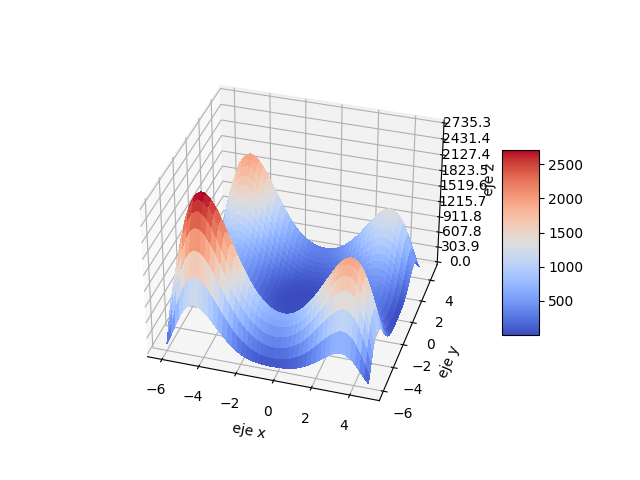
\includegraphics[scale=.4]{3D.png}(a)
    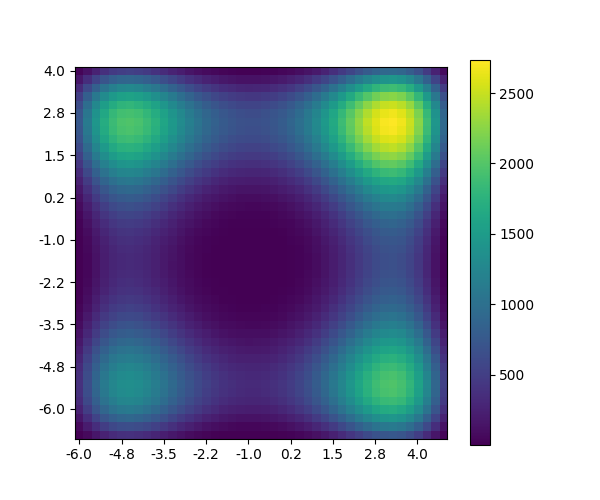
\includegraphics[scale=.4]{2D.png}(b)
    \caption{a)Función graficada en tres dimensiones. b)Función de tres dimensiones vista superior.}
    \label{f1}
\end{figure}

\section{Metodología}
Para la práctica son dados ejemplos qué se pueden consultar en la página de Schaeffer \cite{elisa} donde se puede representar el movimiento de un punto en rojo a la posición más baja en una función vista en 2 dimensiones, a la cual se modifica de manera qué el punto ahora busque el punto más alto como se puede observar en la figura \ref{f3}.

\begin{figure}[H]
    \centering 
    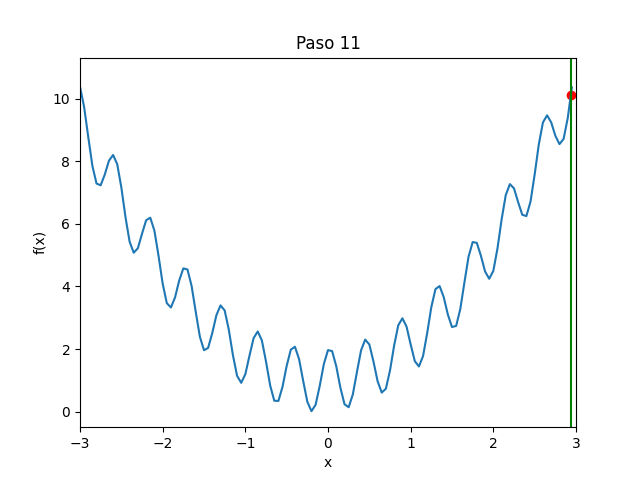
\includegraphics[scale=.4]{Fun_1pt.png}
    \caption{Función dos dimensiones un solo punto.}
    \label{f3}
\end{figure}

La siguiente variante dada en la página \cite{elisa} es generar varios puntos a lo largo de la función que estarán buscando el punto más alto a un número de réplicas dado para lograr visualizar en que replica coinciden todos en el mismo punto, las siguientes figuras \ref{f4} a y b muestran el comportamiento.

\begin{figure}[H]
    \centering 
    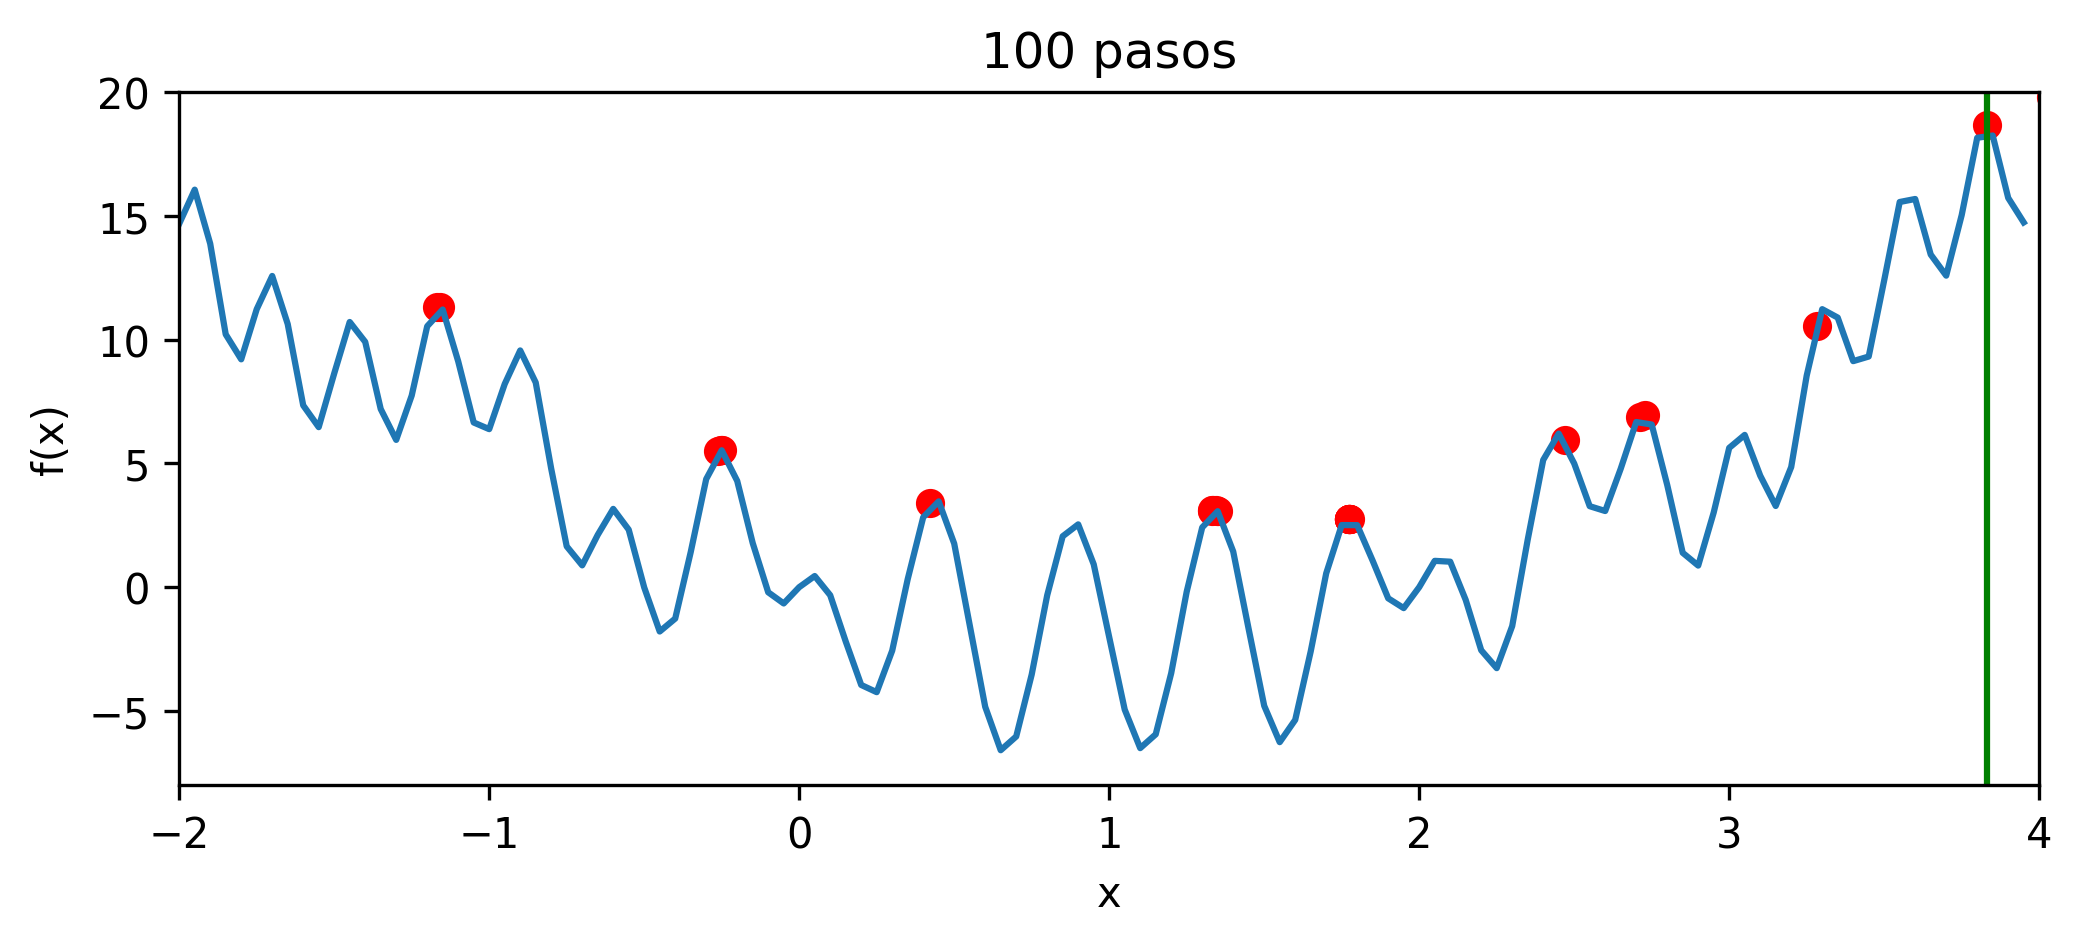
\includegraphics[scale=.4]{fun_varios.png}(a)
    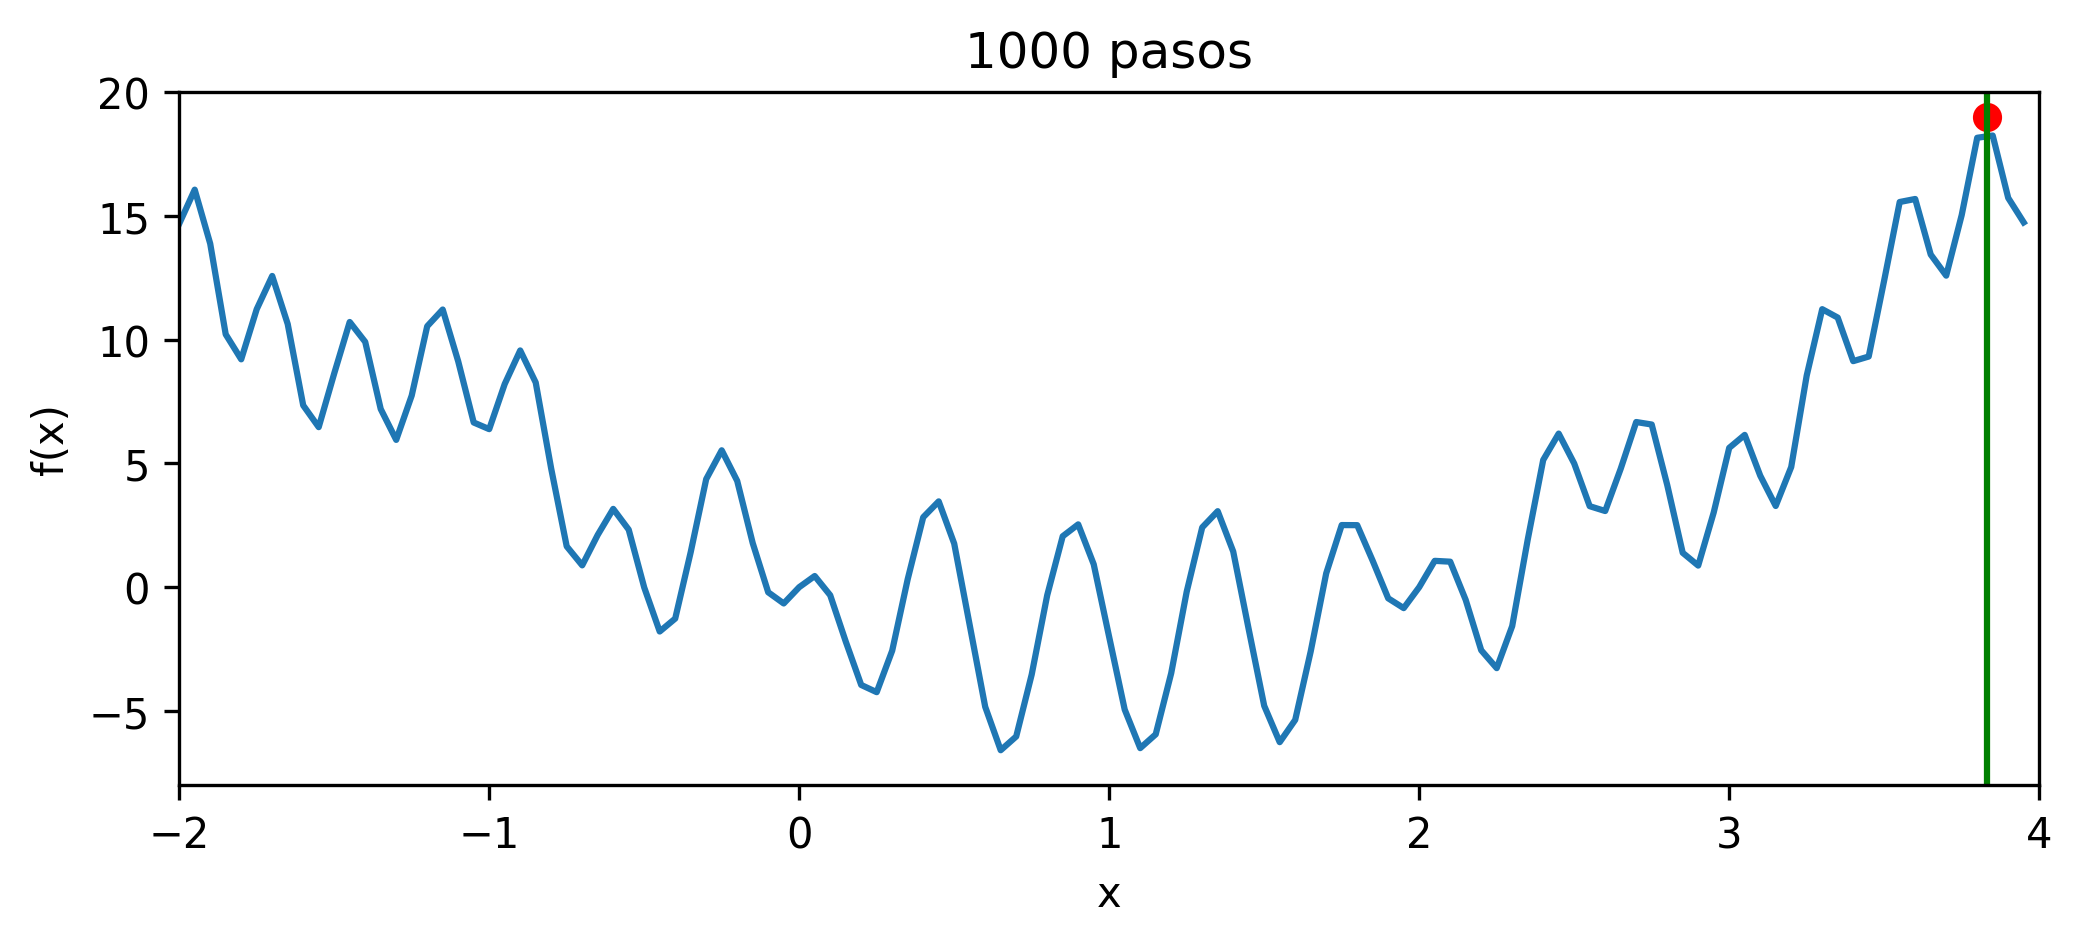
\includegraphics[scale=.4]{fun_1000.png}(b)
    \caption{Función dos dimensiones con varios puntos y replicas.}
    \label{f4}
\end{figure}

\section{Objetivo}

El objetivo principal es crear una visualización animada de cómo proceden quince réplicas simultáneas de la búsqueda con la lógica modificada anteriormente, se realiza este comportamiento en la gráfica en tres dimensiones visualizada desde la parte superior ya que si se utiliza en tres dimensiones los puntos no se apreciarían de la mejor manera.

\section{Simulación}
La programación es modificación del programa dado por Schaeffer \cite{elisa} y el programa puede ser consultado en el github de Samaniego \cite{Edson}.
La primera parte modificada en el programa es el ciclo \texttt{for} inicial en el que contiene treinta ciclos y dentro de el se declara dos variables \texttt{currx y curry} que dan un número al azar entre \texttt{low y high} para los dos ejes y dos variables mas llamadas \texttt{bestx y besty} almacenarán las variables anteriores respectivamente. Posteriormente entra a un ciclo \texttt{for} mas que realiza otras 30 iteraciones por cada ciclo del for global. Esta lógica realiza el camino de un punto, treinta iteraciones y al siguiente ciclo sera el camino de otro punto y así sucesivamente treinta puntos.

\begin{verbatim}
for ciclo in range(tmax):
    
    currx = uniform(low, high)
    curry = uniform(low, high)
    [bestx, besty] = [currx, curry]
    for iteracion in range(tmax):
    
\end{verbatim}

Dentro del segundo ciclo lo que se realiza es determinar los movimientos de izquierda, derecha, arriba y abajo respectivamente a cada eje \texttt{x} y \texttt{y}, restando \texttt{deltax} siendo un dato al azar entre cero y paso qué vale 0.20 qué es el máximo avance por punto, este dato se le resta a la variable \texttt{currx y curry} qué es la posición donde estará el punto. 
Para cada una de las cuatro posiciones se limitan con funciones \texttt{if} para que no sobrepasen los rangos de la gráfica. 

\begin{verbatim}
        deltax = uniform(0, step)
        leftx = currx - deltax  
        leftx = low if leftx < low else leftx  
        rightx = currx + deltax 
        rightx = high if rightx > high else rightx
        
        deltay = uniform(0, step)
        lefty = curry - deltay  
        lefty = low if lefty < low else lefty  
        righty = curry + deltay  
        righty = high if righty > high else righty 
\end{verbatim}

La función \texttt{if} que se ve a continuación, decide sí \texttt{currx y curry} en la función \texttt{g} generada es mayor a \texttt{bestx y besty} en la función g entonces estas ultimas variables tomaran el valor de \texttt{currx curry}.

\begin{verbatim}
        if g(currx, curry) > g(bestx, besty):
            [bestx, besty] = [currx, curry]
\end{verbatim}
De esta manera se asegura que la posición a la que se moverá el punto en la función será una mejor posición y va a tender a una posición más alta sin que descienda.
La última parte de la programación solo consiste en como graficar estos resultados en réplicas de como se desplazan los puntos, se puede consultar en github \cite{Edson}.

\section{Resultados}
Los resultados de la programación archiva imágenes de las réplicas las cuales fueron tomadas para crear un gif con la página Giphy \cite{GIPHY} y puede ser visualizado en github \cite{Edson}.
El inicio del gif se puede observar en la figura \ref{f5}a, en el qué se visualiza como se distribuyen los puntos a lo largo de la función de manera al azar. Para el último paso o réplica del gif es mostrada en la figura \ref{f5}b, se observa que los puntos tienden a irse a los picos más altos en la gráfica siendo el más alto del lado superior derecho.

\begin{figure}[H]
  \centering      
  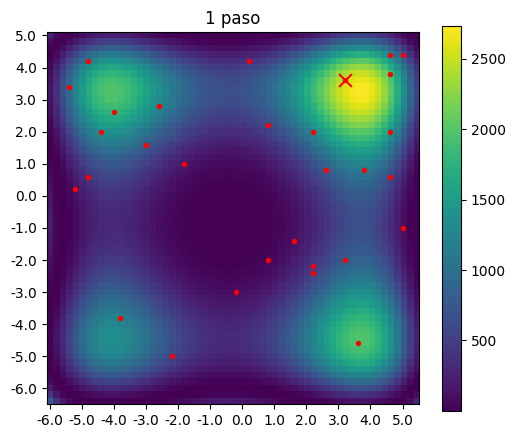
\includegraphics[scale=.6]{p7p_0.png}(a)
  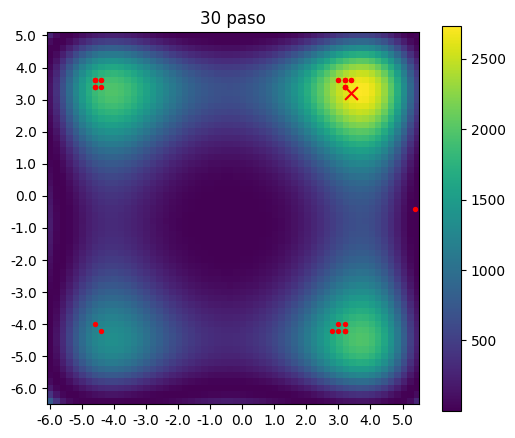
\includegraphics[scale=.6]{p7p_29.png}(b)
  \caption{a) Primera distribución de puntos. b) Paso final con puntos aglomerados en puntos altos.}
  \label{f5}
\end{figure}

\section{Conclusión}
La tendencia de cada punto a ir al pico alto dependerá mucho de en que posición inicien al azar porque sí el punto cae muy cerca en cualquiera de los cuatro picos su tendencia es ir hacia el pico mas cercano aún qué no sea el más alto de los cuatro picos, de esta manera la mayoría de los puntos están en estos cuatro puntos y teniendo una mayor cantidad de puntos rojos en el pico mayor.

\bibliography{refe}
\bibliographystyle{plainnat}

\end{document}